\subsection{Dataset}

Next, we apply our method to brain imaging data from the anonymized multimodal
neuroimaging ``Mother Of all Unification Studies'' (MOUS) dataset \cite{schoffelen2019204}.
The dataset contains magneto-encephalography (MEG) recordings of 102 healthy native-Dutch
adults who participated in a reading task.

Subjects were exposed to a rapid serial visual presentation of Dutch words. The word lists
consisted of 120 sentences, and scrambled lists of the same words. Each word was presented on the computer screen for 351ms on average (min: 300ms, max: 1400ms).
Successive words were separated by a blank screen for 300ms, and successive
sentences were separated by an empty screen for a few (3-4) seconds.

\subsection{MEG preprocessing}

The raw MEG data was bandpass-filtered between 0.1 and 40 Hz using MNE-Python default
parameters \cite{mne}. Specifically, we used a zero-phase finite impulse response filter (FIR) with a hamming window and with transition bands of 0.1 Hz and 10 Hz for the low and high
cut-off frequencies respectively.

The raw data was then segmented 100 ms before word onset and 1.000 sec after
word onset. Time $t=0$ms corresponds to the word onset. Finally, each resulting segment was baseline-corrected between -100ms and 0ms, and decimated by 5 and thus led a sampling frequency of 240 Hz. We show, in Figure \ref{fig:megavg}, the average response of the
magnetometers evoked by the words presented to the first subject.

For each word, each subject, and each time sample relative to word onset, we build an observation matrix $Y \in \mathbb{R}^{n, q}$ of $n\approx$ 2700 words by $q=301$ MEG channels (273 magnetometers and 28 compensation channels). Each of the columns of $Y$ is normalized to have zero mean and unit variance.

\begin{figure}
  \centering
  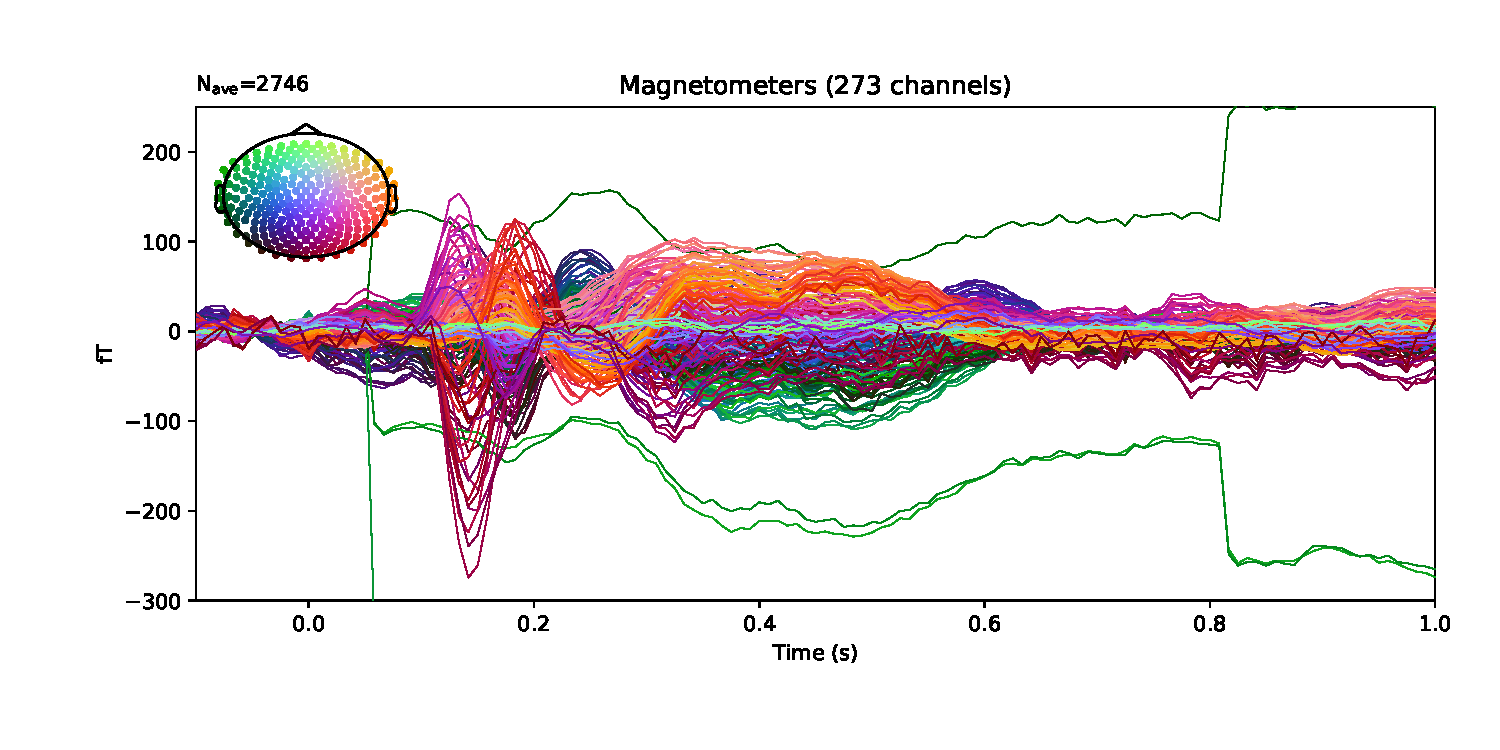
\includegraphics[width=\textwidth, trim=1.5cm 1cm 0.5cm 0cm, clip=True]{figure_meg.pdf}
  \caption{Average magnetosensor response across words for one subject.}
  \label{fig:megavg}
\end{figure}

\subsection{Word features}
We annotated each word with 38 features: 26 corresponds to the number of each letter in the word (from 'a' to 'z', independently of their case), the total number of letters ('word length'), the frequency of the word in natural language (using the Zipf logarithmic scale \cite{marc_brysbaert}), and the part-of-speech tags (i.e. NOUN, PROPN (proper noun), VERB, PRON (pronoun), CONJ (conjunction), DET (determinant), ADJ (adjective), ADV (adverb), and NUM (numerical)) using the packages Spacy \cite{spacy} and WordFreq \cite{speer}. For clarity purposes, we refer to these features using two broad categories: visual (i.e. each letter and the total number of letters) and lexical (part-of-speech and word frequency).
This procedure yields an $X \in \mathbb{R}^{n, d}$ matrix of $n\approx$ 2700 words by $d=38$ features for each subject. Each of the columns of $X$ is normalized to have a mean and a standard deviation of 0 and 1 respectively.

\subsection{Analyses}
We aimed to identify which factors of $X$ explain the MEG recordings $Y$ at each time sample and for each subject separately. To this aim, we implemented three types of analyses (forward, backward and back-to-back regressions), and tested whether their results were consistent across subjects, using a second-level statistics described below.

Forward regression, also known as 'encoding' in neuroimaging, here consisted in fitting a Ridge-regularized OLS from $X$ to $Y$:
\begin{equation}
H = (X^{T}X+\lambda I)^{-1} X^{T}Y
\end{equation}
where $\lambda$ is the regularization parameter fit with the leave-one-out cross-validation implemented in scikit-learn \cite{sklearn} from 20 possible value logarithmatically distributed between $10^{-5}$ and $10^5$. We aimed to estimate the contribution $diag(\hat E) \in\mathbb{D}^{d} $ of each factor. However, $H\in\mathbb{R}^{d, q}$ is a matrix of $d$ word features by $q$ MEG channels. We thus approximated the relative contribution of each feature by sum-squarring the H coefficients:
\begin{equation}
\hat e_d = \sum_{i=0}^{i=q} {h_d^i}^2
\end{equation}


Backward regression, also known as 'decoding' in neuroimaging, here consisted in fitting a Ridge-regularized OLS from $Y$ to $X$:

\begin{equation}
G = (Y^{T}Y+\lambda I)^{-1} Y^{T}X
\end{equation}

where $\lambda$ is the regularization parameter fit with the leave-one-out cross-validation
implemented in scikit-learn \cite{sklearn} from 20 possible value logarithmically distributed
between $10^{-5}$ and $10^5$. We aimed to estimate the contribution $diag(\hat E)
\in\mathbb{D}^{d} $ of each factor. Using 10-fold cross-validation, we thus assessed the ability
of this ridge regression to predict independent and identically distributed data:

\begin{equation}
\hat X_{test} = Y_{test}\cdot G_{train}
\end{equation}

and assessing, for each factor of X independently, the Pearson correlation coefficient $r$ between $X_{test}$ and $\hat X_{test}$ for each cross-validation split.

Finally, we adapted back-to-back regression with two changes. First, to avoid getting a slightly positively-biased estimate of the factors contributing to the MEG signal, we swap the Tikhonov regularization of the first regression $G$ with a trunkated regularization. Trunkation was fitted by maximum likelihood estimate, as implemented in scikit-learn principal component analysis. Second, to minimize the variance increase induced by bagging, we computed the inverse regularized covariance matrices outside bagging:
\begin{equation}
G = (Y_^T Y+\lambda_Y I)^{-1} Y_i^T X_i
\end{equation}

\begin{equation}
\hat X_j = Y_j \cdot G^T
\end{equation}
where i and j are partition of the data.


\subsection{Second-level statistics}

The three types of analyses were implemented for each subject and each time sample independently.
To estimate the reliability of these estimates in the population, we tested, using one-sample t-test whether the distribution of the estimated contribution of each factor different from baseline ($t=-100$ms):

\begin{equation}
ttest(\hat E_{t=-100} - \hat E_{\tau})
\end{equation}
with $\tau \in $ 150ms and 400ms respectively


\subsection{Results}

We aimed to estimate

We show these coefficients as a function of time in the stacked plots, in Figure
\ref{fig:megresult}.

\begin{figure}
  \centering
  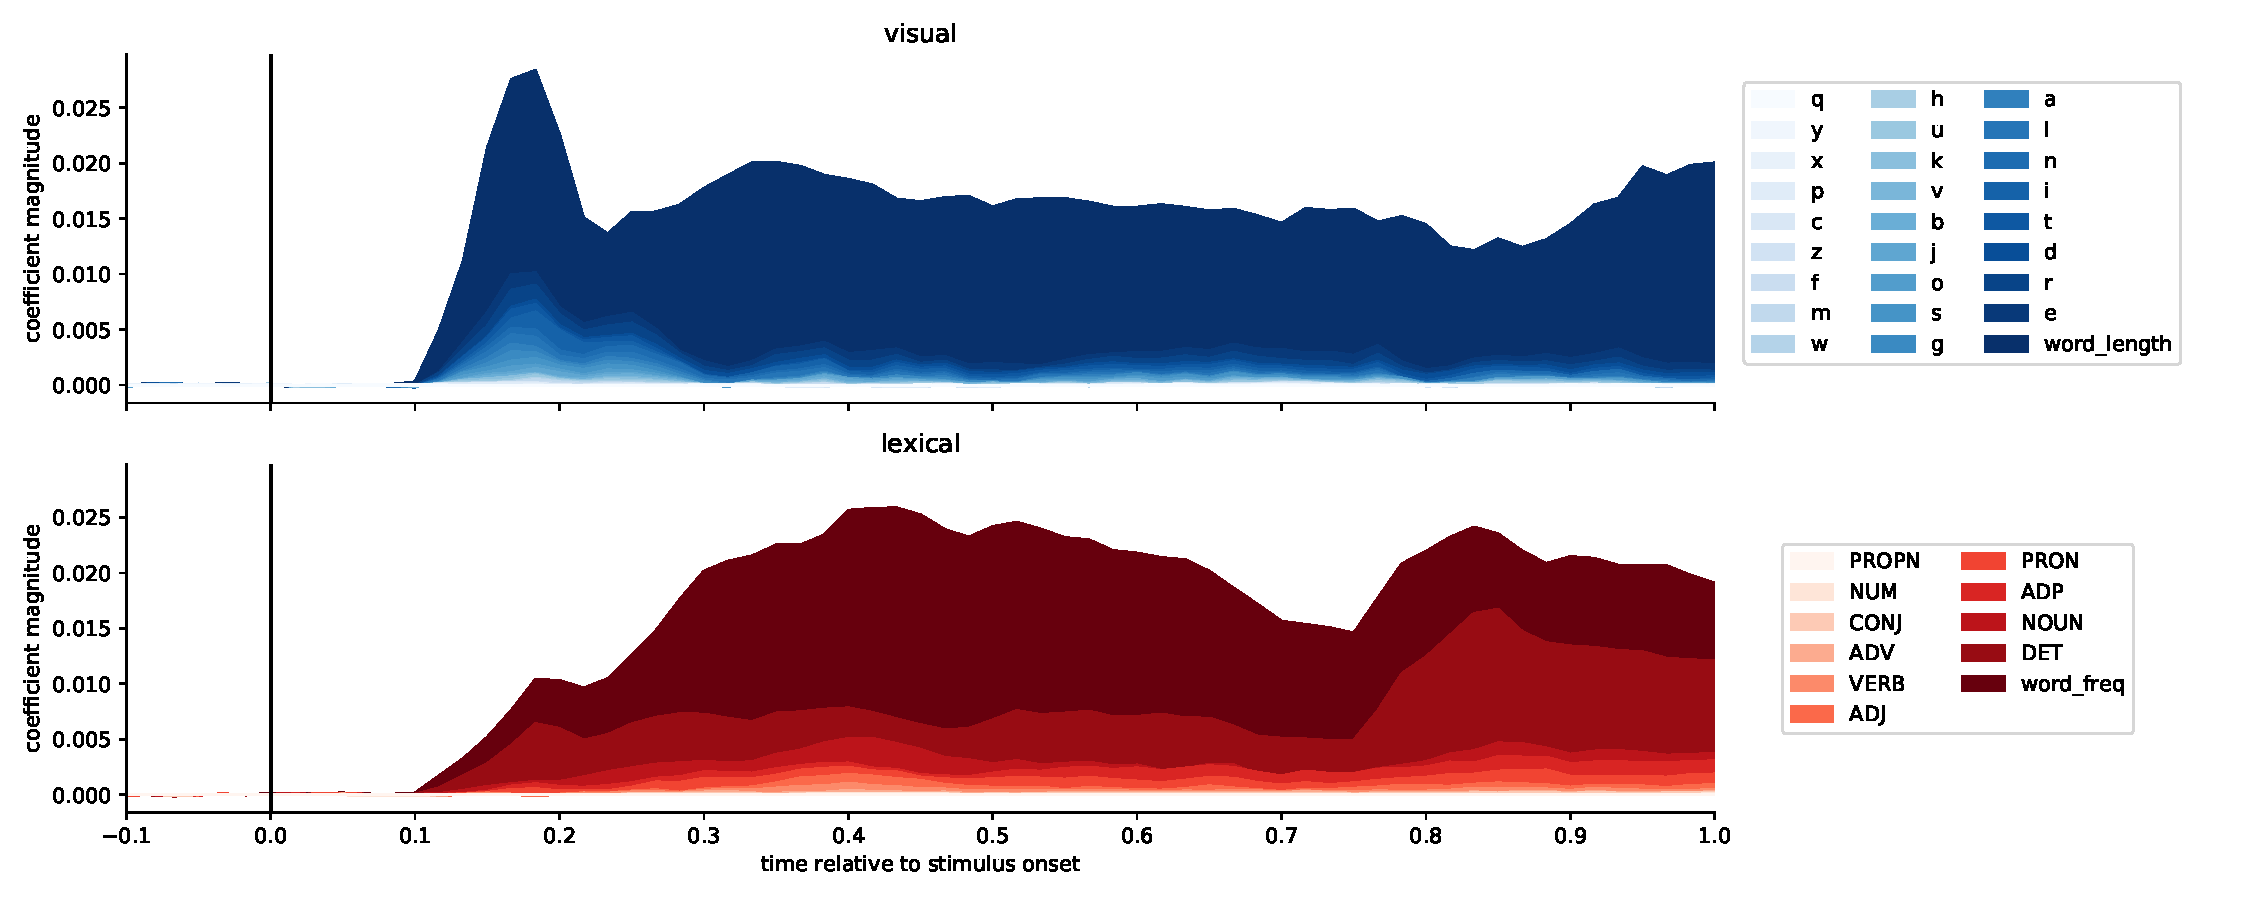
\includegraphics[width=\textwidth, trim=1.5cm 1cm 0.5cm 0cm,
clip=True]{meg_result.pdf}
  \caption{Average magnetosensor response across words for one subject.}
  \label{fig:megresult}
\end{figure}



\subsection{Discussion of the results.}

\subsubsection{Overview}
